\documentclass[8pt, a4paper]{mpscheatsheet}
% mathbox around math statements
% PRE: #1 math expression
\newcommand{\mathbox}[2][]{
    \vskip4pt
    \begin{center}
        \boxed{
            #2
        } #1
    \end{center}
    
    \vskip4pt
}
\usepackage{amsmath, physics}
\usepackage{empheq} % border for align env
\usepackage{cancel}
\usepackage[version=4]{mhchem}
\usepackage[hidelinks]{hyperref}

\title{System Modeling}
\author{Micha Bosshart - bmicha@ethz.ch}

% reduce whitespace above and below equations
\AtBeginDocument{
    \setlength{\abovedisplayskip}{3pt plus 1pt minus 1pt}
    \setlength{\belowdisplayskip}{3pt plus 1pt minus 1pt}
}

\begin{document}
    \section{Systemmodeling for Control}
        \subsection{Definitions}
    \subsubsection{(Non) Parametric Models}
        \textbf{Parametric Models} (Grey/ White Box Models)
        \begin{itemize}
            \item \textit{Forward Formulation}:\\
                Respecting physical causality $\rightarrow$  ODE
            \item \textit{Backward Formulation}:\\
                Optimization problems $\rightarrow$ given velocity, \dots
        \end{itemize}
        \textbf{Nonparametric Models} (Black Box Models)
        \begin{itemize}
            \item Based on experiments $\rightarrow$ Impulse response, \dots
        \end{itemize}
    \subsubsection{Relevant Dynamic Phenomena}
        \begin{minipage}{0.45\linewidth}
            \begin{center}
                \resizebox{\linewidth}{!}{
                \includegraphics[
                        page = {18},
                        trim = {6.7cm, 21.3cm, 7.1cm, 3.2cm}, %l b r t
                        clip
                    ]{external/Skript.pdf}
                }   
            \end{center}
        \end{minipage}
        \begin{minipage}{0.5\linewidth}
            \begin{enumerate}[label=\alph*)]
                \item \textbf{fast} / algebraic
                \item \textbf{relevant} / dynamic
                \item \textbf{slow} / constant
            \end{enumerate}
        \end{minipage}
        
        
        
    

        %!TEX root=ZF_bmicha_SysMod.tex
\subsection{Reservoir-Based Approach}
    \begin{enumerate}
        \item Define \textbf{system boundaries}.
        \begin{itemize}[label=-]
            \item Inputs: What you can control (+ disturbances)
            \item Outputs: What you can measure
        \end{itemize}
        \item Identify \textbf{relevant reservoirs} (mass, energy, information) and the corresponding \textbf{level variables}.
        \item Formulate the \textbf{differential equations} (conservation laws) for all relevant reservoirs.
        $$
            \frac{d}{dt} (\textrm{reservoir content}) = \sum \textrm{inflows} - \sum \textrm{outflows}
        $$
        \item Formulate \textbf{algebraic relations} that express the \textit{flows between the reservoirs} as functions of the level variables.
        \item Resolve implicit \textbf{alg. loops}. $U = U(I), I = I(U)$
        \item Identify \textbf{unknown system parameters}.
        \item \textbf{Validate} the model.
    \end{enumerate}
        \subsection{Causality Diagrams}
    \begin{minipage}{0.52\linewidth}
        \begin{center}
            \resizebox{0.7\linewidth}{!}{
                \includegraphics[
                    page = {9},
                    trim = {3cm, 2cm, 22.4cm, 5.5cm}, %l b r t
                    clip
                ]{Systemmodeling-for-Control/SlidesEx01.pdf}
            }
        \end{center}
    \end{minipage}
    \begin{minipage}{0.47\linewidth}
        \begin{center}
            \resizebox{0.7\linewidth}{!}{
            \includegraphics[
                    page = {9},
                    trim = {12.7cm, 1.8cm, 13.7cm, 5.7cm}, %l b r t
                    clip
                ]{Systemmodeling-for-Control/SlidesEx01.pdf}
            }
        \end{center}
    \end{minipage}
    
    \section{Mechanical Systems}
        
%!Tex root=ZF_bmicha_SysMod.tex 
\subsection{Constraints}
    does \textbf{not} depend on $\dot{q}(t)$ $\rightarrow$ \textbf{holonomic}
    \begin{itemize}
        \item holonomic: $f(\vec{q},t) = 0$
        \item non-holonomic: $f(\vec{q}, \dot{\vec{q}},t) = 0$
    \end{itemize}
\subsection{Energy and Forces}
    \subsubsection{LMB and AMB}
        \textbf{Linear Momentum Balance}
        $$
            \sum \boldsymbol{F} = m \cdot \frac{d}{dt} \boldsymbol{v}(t), \qquad m \neq m(t)
        $$
        \textbf{Angular Momentum Balance} \hfill ($\Theta \ddot{\varphi} = \sum M$)
        \begin{align*}
            \sum \boldsymbol{M}_B &= \boldsymbol{\dot{H}}_B + \boldsymbol{v}_B \times \boldsymbol{P}\\
        \end{align*}
        \vspace{-3em}
        \begin{align*}
            \boldsymbol{H}_B &= \boldsymbol{r}_{BP} \times \boldsymbol{P} && \boldsymbol{P} = m \cdot \boldsymbol{v}_P
        \end{align*}
        % \vspace{-1em}
        % \begin{align*}
        %     \sum F &= m \cdot a &\qquad \sum M &= \Theta \cdot  \ddot{\varphi}
        % \end{align*}
    \subsubsection{Kinetic Energy}
        \mathbox{
            T = \frac{1}{2} m \boldsymbol{v}_p^T \boldsymbol{v}_p + m \boldsymbol{v}_p^T (\boldsymbol{\Omega} \times \boldsymbol{r}_{PS}) + \frac{1}{2} \boldsymbol{\Omega}^T \Theta_P \boldsymbol{\Omega}
        }
        \vspace{-1em}
        \begin{minipage}{0.69\linewidth}
            \textbf{Translational Energy:}
            $$
                T_t = \frac{1}{2} \cdot m \cdot v^2
            $$
            \textbf{Rotational Energy:}
            $$
                T_r = \frac{1}{2} \cdot \Theta \cdot \omega^2
            $$
        \end{minipage}
        \begin{minipage}{0.3\linewidth}
            \begin{center}
                \resizebox{0.9\linewidth}{!}{
                \includegraphics[
                        page = {4},
                        trim = {18cm, 7.5cm, 1.5cm, 3.5cm}, %l b r t
                        clip
                    ]{Mechanical-Systems/Lecture_3a.pdf}
                }
            \end{center}
        \end{minipage}
    \subsubsection{Potential Energy}
        Sole function of the state. Does not depend on path.
        \textbf{Gravitational Energy:}
        $$
            U_g = m \cdot g \cdot h
        $$\vspace{-0.25em}
        \textbf{Linear Spring:}\vspace{-0.25em}
        $$
            U_s = \frac{1}{2} \cdot k \cdot \Delta x^2
        $$
        \textbf{Torsional Spring:}\vspace{-0.25em}
        $$
            U_s = \frac{1}{2} \cdot k \cdot \Delta \varphi^2
        $$
    \subsubsection{Resistance Forces}
        \begin{minipage}{0.7\linewidth}
            \vspace{2pt}
            \textbf{Air Resistance:}
            \mathbox{
                F = \frac{1}{2} \cdot \rho \cdot A \cdot c_w \cdot v_{rel}^2(t)
            }
            \begin{itemize}[label=-]
                \item $A$: Projected Area
                \item $v_{rel}$: relative vel. object $\leftrightarrow$ air
                \item  $c_w$: drag coefficient
            \end{itemize}
            \vskip3pt
            \textbf{Rolling Resistance:}
            \mathbox{
                F = c_r \cdot m \cdot g
            }
        \end{minipage}
        \begin{minipage}{0.29\linewidth}
            \begin{center}
                \resizebox{\linewidth}{!}{
                    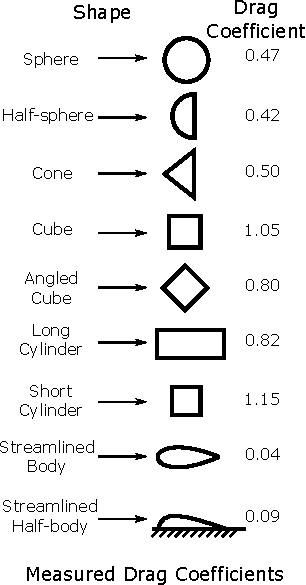
\includegraphics{Mechanical-Systems/drag-coefficient.pdf}
                }
            \end{center}
        \end{minipage}
        \vspace{-0.5em}
    \subsubsection{Conservative Forces}
        $
            F = - \grad U %- \frac{\partial U^T}{\partial q}
        $ : gradient of a potential function
       
    \subsection{Euler Method}
        \vspace{-1em}
        \begin{align*}
            E(t) &= T(t) + U(t) &\quad \frac{d}{dt}E(t) &= \sum_{i=1}^k P_i(t)
        \end{align*}

        \begin{itemize}
            \item  \textbf{Power $P$ of a Force}: \phantom{o} \boxed{P_F = \vec{F} \cdot \vec{v}}
            \item  \textbf{Power $P$ of a Torque}: \boxed{P_T = \vec{T} \cdot \vec{\omega}}
        \end{itemize}
    
       

            
            

        \subsection{Moment of Inertia}
    \begin{center}
        \resizebox{0.7\linewidth}{!}{
        \includegraphics[
                % page = {4},
                % trim = {18cm, 7.5cm, 1.5cm, 3.5cm}, %l b r t
                % clip
            ]{Mechanical-Systems/moment-of-inertia.png}
        }
    \end{center}
    \subsubsubsection{Parallel Axis/ Steiner's Theorem}
        \vskip4pt
        \mathbox{
            I_A = I_{CM} + m\cdot d^2
        }
        \subsection{Lagrange Formalism}
    \begin{enumerate}
        % \item Identify generalized coordinates $q_i$.
        % \item Define \textbf{kinetic} $T(q,\dot{q})$ and \textbf{potential} $U(q)$ energy.
        \item Define Lagrange function
            \mathbox{
                L(q,\dot{q}) = T((q,\dot{q})) - U(q)
            }
        \item Determine \textbf{generalized forces} $Q_i$\\[1em]
            \begin{minipage}{0.48\linewidth}
                \centering\underline{Force}
                \begin{empheq}[box=\fbox]{align*}
                    v_A &= J_A \cdot \dot{q} + \xi_A\\
                    Q_A &= J_A^T \cdot F_A
                \end{empheq}
                \begin{itemize}
                    \item[] $v_A$: velocity in $A$ 
                    \item[] $J_A$: Jacobian in $A$
                    \item[] $\xi_A$: offset term
                    \item[] $F_A$: Force in $A$
                \end{itemize}
            \end{minipage}
            \begin{minipage}{0.5\linewidth}
                \centering\underline{Torque}
                \begin{empheq}[box=\fbox]{align*}
                    \omega_B &= J_B \cdot \dot{q} + \xi_B\\
                    Q_B &= J_B^T \cdot M_B
                \end{empheq}
                \begin{itemize}
                    \item[] $\omega_B$: ang.vel. in $B$ 
                    \item[] $J_B$: Jacobian in $B$
                    \item[] $\xi_B$: offset term
                    \item[] $M_B$: Torque in $B$
                \end{itemize}
            \end{minipage}
            \vspace{2pt}
        \item Generate system of equations\\
            - \underline{\textbf{Without} kinematic constraints}:
            \vspace{-4pt}
            \mathbox[$\ i = 1, \dots, 3n-k$]{
                \frac{d}{dt} \left\{ \frac{\partial L}{\partial \dot{q}_i} \right\} - \frac{\partial L}{\partial q_i} = Q_i
            }
            \vspace{-10pt}
            \begin{itemize}
                \item[] $n$: \# rigid bodies
                \item[] $k$: \# holonomic constraints 
            \end{itemize}
            - \underline{\textbf{With} kinematic constraints}:
            \vspace{-4pt}
            \mathbox[$\ i = 1, \dots, n$]{
                \frac{d}{dt} \left\{ \frac{\partial L}{\partial \dot{q}_i} \right\} - \frac{\partial L}{\partial q_i} - \sum\limits_{j=1}^\nu \mu_j \alpha_{j,i}= Q_i
            }
            \vspace{-2em}
            \mathbox{
                \alpha^T_j \cdot \dot{q} = 0
            }
            \vspace{-10pt}
            \begin{itemize}
                \item[] $\to$ $\nu$ \textbf{additional} eqn's :  $\alpha^T_j \cdot \ddot{q} = 0$
                \item[] $\nu$: \# non-holonomic contraints
            \end{itemize}

        \item implicit $\rightarrow$ explicit \hfill $\left(M = M^T\right)$
            \begin{align*}
                M(q) \cdot \ddot{q} = f(q,\dot{q},u)&  &\Rightarrow& &\ddot{q} =  M(q)^{-1} \cdot f(q,\dot{q},u)
            \end{align*}
        \vfill \null

    \end{enumerate}
    \section{Hydraulic Systems}
        %!TEX root=ZR_bmicha_SysMod.tex

\subsection{Hydraulic Duct}
    \begin{minipage}{0.67\linewidth}
        \begin{center}
            \resizebox{\linewidth}{!}{
            \includegraphics[
                    page = {36},
                    trim = {6.5cm, 11cm, 6.5cm, 11.5cm}, %l b r t
                    clip
                ]{External/Skript.pdf}
            }
        \end{center}
    \end{minipage}
    \begin{minipage}{0.31\linewidth}
        \begin{center}
            \resizebox{\linewidth}{!}{
            \includegraphics[
                    page = {5},
                    trim = {17cm, 1cm, 9cm, 11.25cm}, %l b r t
                    clip
                ]{Hydraulic-Systems/SlidesEx02.pdf}
            }
        \end{center}       
    \end{minipage}
    \textbf{Newton's Law} yields:
    \mathbox{
        \frac{d}{dt}v(t) = \frac{1}{\rho l} (p_1(t) - p_2(t)) + \frac{g h}{l} - \frac{F_{fric}(t)}{\rho l A}
    }
    $$
        F_{fric}(t) = A \cdot \lambda(v(t)) \cdot \frac{l}{d} \cdot \frac{\rho}{2} \cdot v^2(t) \cdot sgn(v(t))
    $$
\subsection{Compressible Duct}
    \begin{minipage}{0.68\linewidth}
        \begin{center}
            \resizebox{\linewidth}{!}{
            \includegraphics[
                    page = {37},
                    trim = {7cm, 13cm, 7cm, 12cm}, %l b r t
                    clip
                ]{External/Skript.pdf}
            }
        \end{center}
    \end{minipage}
    \begin{minipage}{0.31\linewidth}
        \begin{center}
            \resizebox{\linewidth}{!}{
            \includegraphics[
                    page = {8},
                    trim = {17cm, 1cm, 9cm, 11.5cm}, %l b r t
                    clip
                ]{Hydraulic-Systems/SlidesEx02.pdf}
            }
        \end{center}       
    \end{minipage}
    
    \mathbox{
        \frac{d}{dt}V(t) = \dot{V}_{in} - \dot{V}_{out} = A_{in} \cdot v_{in} - A_{out} \cdot v_{out}
    }
    \mathbox{
        p(t) = \frac{1}{\sigma_0} \cdot \frac{V(t) - V_0}{V_0} + p_{static}
    }
    $$
        \sigma_0 = \frac{1}{V_0} \cdot \frac{dV}{dp} \qquad \left[\frac{1}{Pa}\right]
    $$
\subsection{Valve}
    \vspace{-1em}
    \begin{center}
        \resizebox{\linewidth}{!}{
            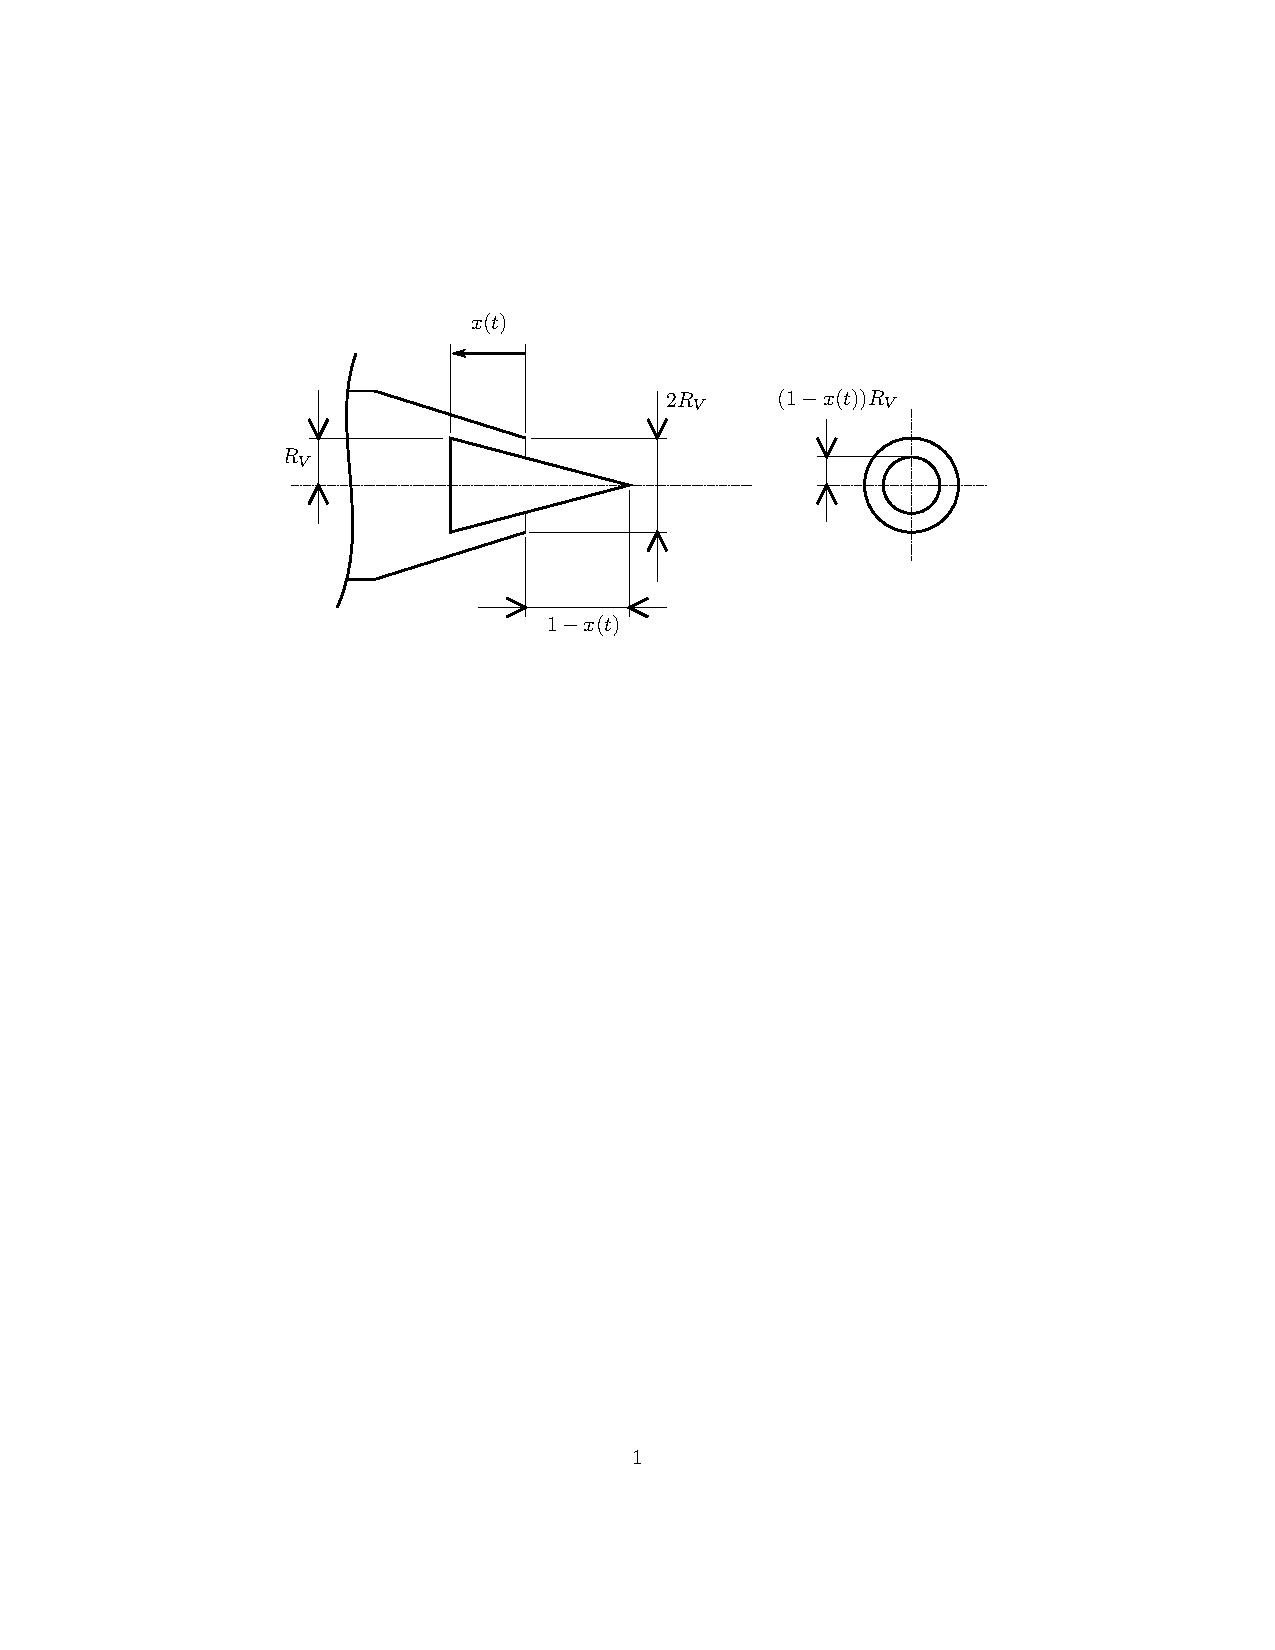
\includegraphics[
                page = {1},
                trim = {4cm, 17cm, 5cm, 5cm}, %l b r t
                clip
            ]{Hydraulic-Systems/valve.pdf}
        }
    \end{center}
    \textbf{Opening Area of the Valve:}
    \begin{align*}
        A_V(t) &= \pi \cdot R_V^2 - \pi \cdot \left( (1-x(t)) \cdot R_V\right)^2\\
        &= A_{V0} \cdot \left( 1 - (1-x(t))^2 \right)
    \end{align*}
    \textbf{Flow Velocity of \textit{Incompressible} Medium}
    $$
        v_V(t) = c_d \cdot \sqrt{\frac{2 \cdot (p_F(t) - p_0)}{\rho}}, \qquad v_V \gg v_{in}
    $$
        
        \vfill \null \columnbreak
    \section{Electric Systems}
        \subsection{General Laws}
    \begin{itemize}[label=-]
        \item Biot-Savart \& Lorentz
            $$ \boldsymbol{F} = I (\boldsymbol{l} \times \boldsymbol{B}) = q (\boldsymbol{v} \times \boldsymbol{B}) $$
        \item Faraday
            $$ U = - v (\boldsymbol{l} \times \boldsymbol{B})$$
        \item Motor
            $$ T(t) = \kappa \cdot I(t)$$
        \item Generator
            $$ U_{ind}(t) = \kappa \cdot \omega(t)$$
    \end{itemize}

\subsection{Reservoirs \& Energies}
\begin{center}
    \renewcommand{\arraystretch}{1.5}
    \begin{tabular}{l|c|c}
        & Capacitance $C$& Inductance $L$\\
        \hline \hline
        Energy & $W = \frac{1}{2} C U^2$ & $W = \frac{1}{2} L I^2$\\\hline
        Stored in & $\boldsymbol{E}$-Field & $\boldsymbol{B}$-Field\\\hline
        Level Var & U(t) & I(t)\\\hline
        Cons. Law & $C \cdot \frac{d}{dt}U = I$ & $L \cdot \frac{d}{dt}I = U$\\\hline
        Impedance & $Z(s) = \frac{1}{s \cdot C}$ & $Z(s) = s \cdot L$
    \end{tabular}
\end{center}
    \section{Thermodynamic Systems}
        %!Tex root=ZF_bmicha_SysMod.tex
\subsection{Closed Systems}
    \vspace{4pt}
    \hfill \boxed{\Delta E = Q - W}  $\qquad W = \int p \cdot dV$
    % \begin{itemize}
    %     \item $\Delta U = m \cdot c_{v} \cdot \Delta T$
    % \end{itemize}
    % \subsubsection{Incompressible Fluids}
    %     \mathbox{c_p = c_v = c}
    %     % \begin{itemize}
    %     %     \item $\Delta Q = m \cdot c \cdot \Delta T$
    %     % \end{itemize}

\subsection{Open Systems}
    \mathbox{\frac{dE}{dt} = \dot{Q} - \dot{W} + \sum \dot{m}_{in} \cdot h_{in} - \sum \dot{m}_{out} \cdot h_{out}}
    \vspace{-1em}
    % \begin{itemize}
    %     \item $\Delta H = m \cdot c_{p} \cdot \Delta T$
    % \end{itemize}
\subsection{Ideal Gases}
    \vspace{-1em}
    \begin{align*}
        h &= h(T) = m \cdot \int c_p\, d\vartheta\\
        u &= u(T) = m \cdot \int c_v\, d\vartheta\\
        p \cdot V &= n \cdot \bar{R} \cdot \vartheta = m \cdot R \cdot \vartheta\\
        R &= \frac{\bar{R}}{M_{gas}} = c_p - c_v\\
        \bar{R} &= 8.314~\frac{J}{ K \cdot mol } 
    \end{align*}
    \subsubsection{Perfect Gases - (no interatomic forces)}
        \mathbox{c_p = c_v = c = \cancel{c}}
        \vspace{-1em}
    \subsubsection{Isentropic}
        \vspace{-1em}
        \begin{align*}
            p \cdot V^\gamma &= \cancel{c} && \gamma = \frac{c_p}{c_v}\\
            \vartheta \cdot V^{\gamma - 1} &= \cancel{c}\\
            p^{1-\gamma} \cdot \vartheta^\gamma &= \cancel{c}
        \end{align*}
        $\gamma = \frac{5}{3}$, mono-atomic gas; $\gamma = \frac{7}{5}$, di-atomic gas
\subsection{Heat Transfer}
    \begin{center}
        \begin{tabular}{lp{6pt}l}
            Conduction&&$ \overset{*}{Q} = \frac{\kappa \cdot A}{l} \cdot  \Delta \vartheta $\\
            Convection&&$ \overset{*}{Q} = k \cdot A \cdot  \Delta \vartheta $\\
            Radiation&&$ \overset{*}{Q} = \varepsilon \cdot \sigma \cdot A \cdot  \Delta \vartheta $
        \end{tabular}
    \end{center}
    \begin{itemize}
        \item $\kappa\ $ thermal conductivity $\frac{W}{m K}$
        \item $k\ $ heat transfer coefficient $\frac{W}{m^2 K}$
        \item $\varepsilon\ $ emissivity
        \item $\sigma\ $ Stephan-Boltzmann const, $5.67\cdot10^{-8}~\frac{W}{m^2 K^4}$
    \end{itemize}
\subsection{Incompressible Fluids}
    \subsubsubsection{Mass flow through valve}
        \vspace{0.5em}
        $$
            \overset{*}{m}(t) = c_d \cdot A(t) \cdot \sqrt{2\rho} \cdot \sqrt{p_{in}-p_{out}}
        $$
\subsection{Compressible Fluids}
    \subsubsubsection{Mass flow through insenthalpic throttle}
        \vspace{0.5em}
        $$
            \overset{*}{m}(t) = c_d \cdot A(t) \cdot \frac{p_{in}(t)}{\sqrt{R \cdot \vartheta_{in}(t)}} \cdot \Psi(p_{in},p_{out})
        $$
        with
        $$
            \Pi \vcentcolon= \frac{p_{out}}{p_{in}}
        $$
        $$
            \Psi = 
            \begin{cases}
                \sqrt{\kappa \cdot \left( \frac{2}{\kappa + 1} \right)^{\frac{\kappa + 1 }{\kappa -1}}}, \quad \textrm{choked if } \Pi < \left( \frac{2}{\kappa + 1} \right)^{\frac{\kappa}{\kappa - 1}}\\[1em]
                \Pi^{\frac{1}{\kappa}} \cdot \sqrt{\frac{2\kappa}{\kappa -1} \left[ 1 - \Pi^{\frac{\kappa-1}{\kappa}} \right]}, \quad \textrm{subsonic otw}
            \end{cases}
        $$

    \section{Chemical Systems}
        %!Tex root=ZF_bmicha_SysMod.tex
\vspace{-0.5em}
\begin{align*}
    \alpha \ce{A} + \beta \ce{B} \underset{+}{\overset{-}{\ce{<=>}}}\gamma \ce{C} + \delta \ce{D}
\end{align*}
\subsection{Rate of Formation}
Forward ($-$) and Backward ($+$) Reaction:
\begin{align*}
    \frac{d^-}{dt}[A] &= - \alpha \cdot r^- \cdot [A]^\alpha \cdot [B]^\beta\\
    \frac{d^+}{dt}[A] &= \phantom{-} \alpha \cdot r^+ \cdot [C]^\gamma \cdot [D]^\delta
\end{align*}
Total rate of formation for $A$:
$$  
    \frac{d}{dt}[A] = \alpha \left( r^+ \cdot [C]^\gamma [D]^\delta - r^- \cdot [A]^\alpha [B]^\beta \right) \pm \frac{\overset{*}{m}(t)}{V \cdot M}
$$
\subsubsection{Arrheniusmodel}
    $$
        r^\pm = k^\pm (\vartheta, p, \dots) \cdot \exp\left(\frac{-E^\pm}{R \cdot \vartheta}\right)
    $$
    \begin{itemize}[label=-]
        \item $E$: Activation Energy
        \item $R$: Universal Gas Constant
        \item $r$: Reaction constant
    \end{itemize}
        \vfill \null \columnbreak
    \section{Fluiddynamics}
        \subsection{Bernoulli}
    \textbf{Assumptions:}
    \begin{itemize}
        \item conservative forces
        \item incompressible fluid
    \end{itemize}
    \subsubsection{Frictionless Bernoulli}
        \textbf{Assumptions:}
        \begin{itemize}
            \item frictionless $\rightarrow$ valid along streamline
            \item frictionless and $\underline{\nabla} \times \underline{u} = 0$ $\rightarrow$ valid in entire field
        \end{itemize}
        \mathbox{
            \int_1^2 \frac{\partial \underline{u}}{\partial t} \cdot d \underline{s} + \left[ \frac{p}{\rho} + \frac{1}{2} \abs{\underline{u}}^2 + U \right]^2_1 = 0
        }
    \subsubsection{Stationary Bernoulli with Friction}
        \mathbox{
            \frac{p_1}{\rho} + \frac{1}{2} \abs{\underline{u}_1}^2 + g z_1 = \frac{p_2}{\rho} + \frac{1}{2} \abs{\underline{u}_2}^2 + g z_2 + \frac{\Delta p_{12}}{\rho}
        }
        \begin{itemize}
            \item \textbf{Turbulent Pipe Friction}: 
            $$ \frac{\Delta p_{12}}{\rho} = \lambda \frac{L}{D} \frac{\overline{u}^2}{2} $$
            \item \textbf{Installations}:
            $$  \frac{\Delta p_{12}}{\rho} = \zeta \frac{\overline{u}^2}{2}$$
            \item \textbf{Pumps}:
            $$ \Delta p_P = - \frac{\eta N}{\dot{V}} $$
            \item \textbf{Turbines}:
            $$ \Delta p_T = - \frac{N}{\eta \dot{V}} $$
        \end{itemize}
        \vfill \null \columnbreak
    \section{Analysis of Linear Systems}
        \subsection{Linearization}
    \begin{align*}
        \dot{x} &= A \cdot x + B \cdot u &=\vcentcolon f(x)\\
              y &= C \cdot x + D \cdot u &=\vcentcolon g(x)
    \end{align*}
    \begin{align*}
        A_{i,j} = \left. \frac{\partial f_i}{\partial x_j} \right\rvert_{x_0,u_0} && B_{i,j} = \left. \frac{\partial f_i}{\partial u_j} \right\rvert_{x_0,u_0}\\
        C_{i,j} = \left. \frac{\partial g_i}{\partial x_j} \right\rvert_{x_0,u_0} && D_{i,j} = \left. \frac{\partial g_i}{\partial u_j} \right\rvert_{x_0,u_0}
    \end{align*}

    
\end{document}